\section{Encrypted Message Complexity}\label{sec:section6}
In order to determine how secure RSA is, I let $P_i$ denote the $i$th prime number; I then calculate the product of the pairs from the first to the 999th prime number, with each pair calculated individually as follows:
$$
P_1 \times P_2, P_2 \times P_3, P_3 \times P_4, \ldots, \,
P_{999} \times P_{1000}
$$
Each prime pair represents $p,q$ with every product representing $n$. I then encrypt the same message 999 times using all of the prime pairs, which allows me to plot all encrypted outputs vs $P$. This in turn enables me to compare the prime numbers used to their encrypted outputs, which highlights any correlation between prime numbers used and the encrypted output. Correlations between prime factors of $n$ and encypted outputs can be considered vulnerabilities since it would theoretically allow someone to reverse engineer $p$ and $q$ from $c$.

\subsection{Comparison}\label{sec:section6.1} 
In order to accurately measure the impact that prime numbers $p$ and $q$ have on the encrypted output of a message, I encrypt the same message with all $P$ pairs, meaning the output will be altered by the prime numbers used and not the encrypted message. The message I encrypt is “hello” meaning that before I encrypt the message, I need to convert the message to integers using a padding scheme, as outlined in \autoref{sec:section3.2}. The padding scheme I use is the following:

\begin{table}[H]
    \centering
    \caption{Simple Padding Scheme}
   \begin{tabular}{ |p{3cm}|p{3cm}|  }
       \hline
       Character & Number\\
       \hline
       A  &  01 \\
       B  &  02 \\
       C  &  03 \\
       D  &  04 \\
       E  &  05 \\
       F  &  06 \\
       G  &  07 \\
       H  &  08 \\
       I  &  09 \\
       J  &  10 \\
       K  &  11 \\
       L  &  12 \\
       M  &  13 \\
       \hline
   \end{tabular}
   \begin{tabular}{ |p{3cm}|p{3cm}|  }
       \hline
       Character & Number\\
       \hline
       N  &  14 \\
       O  &  15 \\
       P  &  16 \\
       Q  &  17 \\
       R  &  18 \\
       S  &  19 \\
       T  &  20 \\
       U  &  21 \\
       V  &  22 \\
       W  &  23 \\
       X  &  24 \\
       Y  &  25 \\
       Z  &  26 \\
       \hline
   \end{tabular}
   \end{table}

Thus, my message $M$, which was originally “hello” is now converted to $m$ which reads “08 05 12 12 15”. This allows me to encrypt $m$ iteratively, using progressively larger prime factors every iteration. After I have encrypted $m$ with every pair of primes, I plot the encrypted output for every number in $m$ against $P$, which in turn reveals a pattern. Below is the graph for the first number in $m$ (08) compared to $P$.

\begin{figure}[ht]
    \centering
    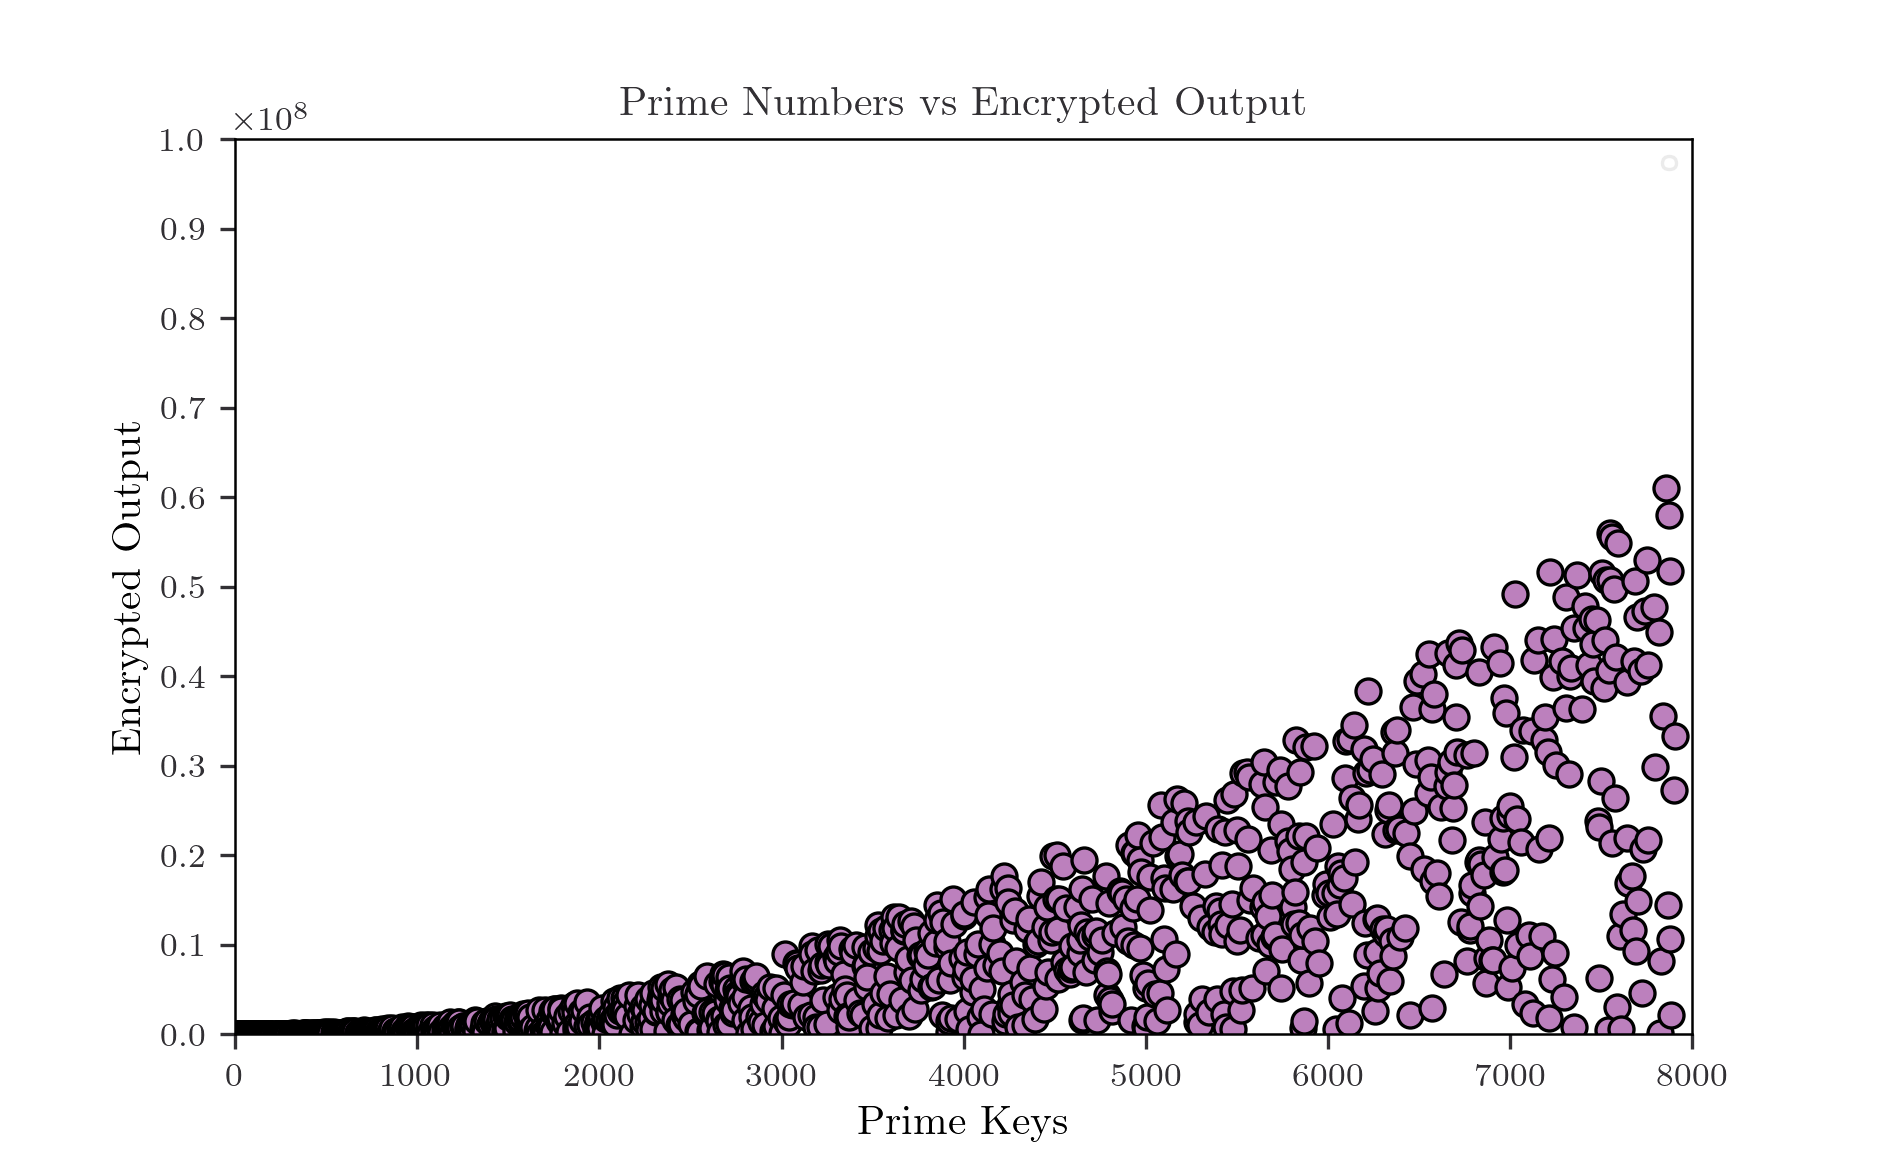
\includegraphics{/comparison/firstterm.png}
\end{figure}

\subsection{Analysis}\label{sec:section6.2}
As seen in the graph above, $p$ and $q$ don't have a direct correlation with the encrypted output since the encrypted message can be any number within a range of values, meaning that it is impossible to determine the prime values used to generate $n$ solely from an encrypted message. That being said, there does appear to be a clear relationship between the primes and encrypted outputs, particularly when it comes to the maximum encrypted output of a message given a range of possible values. The reason why there is a clear maximum value that an encrypted message can have given specific primes is that the encryption process behind RSA uses modulus $n$, specifically 

$$
c \equiv m^{e} \pmod{n}
$$

Whenever you take the modulus of a number, the result is always between 0 and the modulus minus 1. Hence, the maximum value that $c$ can have will always be $n-1$, as $n$ is congruent to $0 \pmod{n}$ and larger numbers will just continue to 'loop' within the modulus $n$. Because of this property, we can plot $P_{n} \cdot P_{n+1} -1$ which represents the maximum possible value for a message that has been encrypted using any pair of prime factors. The graph below highlights possible and impossible encrypted outputs for the first thousand prime pairs.

\begin{figure}[H]
    \centering
    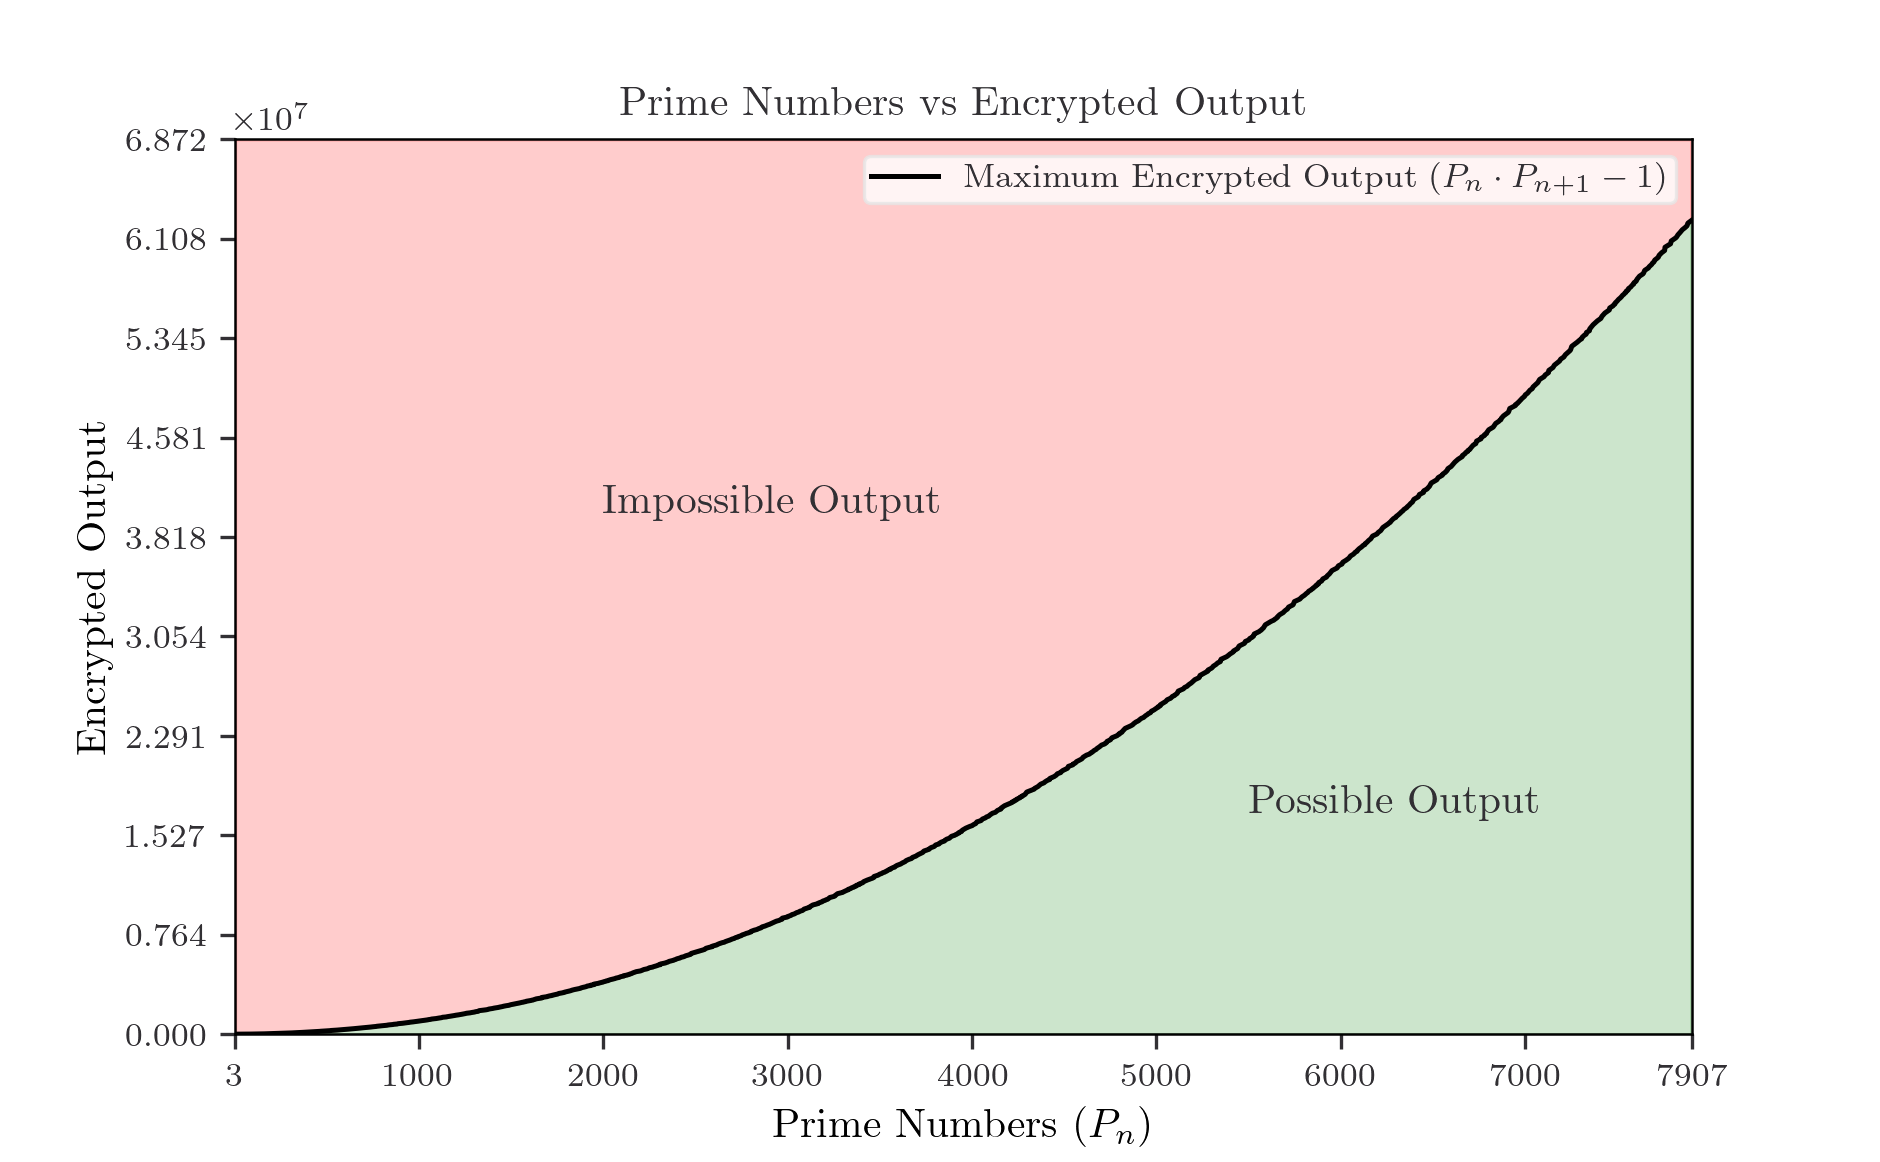
\includegraphics{/comparison/prime_comparison.png}
\end{figure}

The figures above help illustrate how an attacker could exploit mathematical vulnerabilities within RSA in order to determine the private exponent used and decrypt messages.
Firstly, attackers could find $n$ if they used encrypted messages to determine the maximum encrypted output $(n-1)$. While $n$ is part of the public key, it is oftentimes not displayed to users in computer software since the entire RSA encryption and decryption processes happen in the background.
Secondly, using Property (\ref{eq:4}), we know that an attacker could use $n$, more specifically, $\lambda(n)$, to derive $d$ and decrypt messages.

Although both of the aforementioned vulnerabilities that I found in the RSA cryptosystem could be exploited, I concluded that these could be avoided entirely by following a few key generation guidelines. At its core, RSA’s last line of defense relies on its use of prime numbers. While the carmichael function can be used to derive $d$ from $n$, finding it requires one to split $n$ into its two prime factors $(p,q)$. This is straightforward for someone who already knows the values of $p, q$. What about someone who only knows the value of $n$? Assuming that both primes were discarded, and remain unknown, deriving $p$ and $q$ from $n$ could be practically impossible due to prime factorization complexity. Since $n$ is the product of two primes, it has no obvious factors other than $p$ and $q$ themselves. This can make it extremely computationally challenging to factor $n$. Factoring such numbers is done using exhaustive search algorithms; these become increasingly slow as the size of $n$ increases, uncovering two methods to negate the found vulnerabilities.

Firstly, choosing extremely large prime numbers as $p$ and $q$ strengthens the security of RSA, since $n$ will become exponentially larger as $p$ and $q$ grow, creating so many possible encryption values that it would become far too impractical for an attacker to estimate the value of $n$ from encrypted messages. Furthermore, while keeping $n$ hidden would be beneficial in instances where $n$ could be factored, the use of large primes makes this computationally impossible, eliminating the possibility of someone deriving $d$ from $n$.

Secondly, using primes that are significantly different in magnitude makes it too impractical for an attacker to try to find an exact value of $n$. Since larger values result in more primes between $0$ and $n$, testing all permutations of the product of any two primes would be useless when there is no known relationship between $p$ and $q$. In the analysis I conducted, prime factors are always two consecutive primes, meaning they are always a prime number and the next prime number in sequence. I chose to use consecutive primes intentionally, since it clearly demonstrates how the increase in magnitude for both factors contribute to the exponential increase in the range of possible values for $c$. In this instance, it would be obvious that $p$ and $q$ must be of a relatively similar magnitude, since they are consecutive prime numbers. This would enable an attacker to test a significantly smaller range of possible values, since both numbers are known to be consecutive primes near $\sqrt{n}$. In contrast, using primes that are different in magnitude and have been chosen randomly ensures that there is no way to reduce the permutations of $n$ without running the risk of completely skipping the correct pair of prime numbers.